\subsection{Class Hierarchy}

As described in section \ref{section_classes}, the \textit{Controller}, \textit{Repository}, \textit{Model} classes extensively adhere to Inheritance. The concept has been depicted in the figure \ref{fig:controller_hierarchy} for the \textbf{Controller} classes. \\ \\

\begin{figure}[ht]
	\centering
	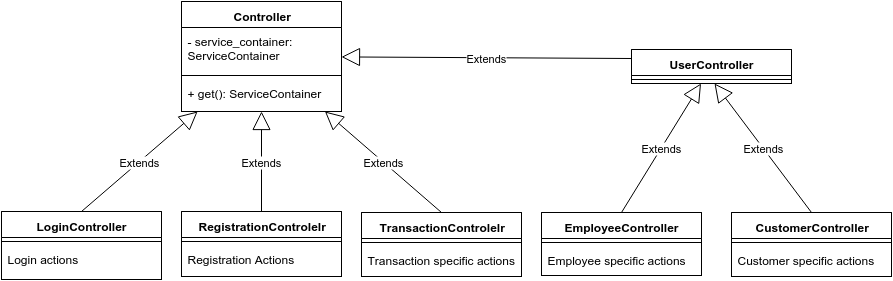
\includegraphics[width=0.9\linewidth]{figures/controller_hierarchy.png}
	\caption{Hierarchy of Controller classes}
	\label{fig:controller_hierarchy}
\end{figure}

\vspace{10mm}

\textbf{Controller} is the Base class for all controllers in the application. All other controllers such as the \textit{UserController}, \textit{LoginController}, \textit{RegistrationController} and \textit{TransactionController} inherit from the base class. 

On a top level, Customer and Employee objects are Users. So all functionality that is applicable to a \textit{User} is also applicable to a \textit{Customer} and an \textit{Exmployee}. Hence the \textit{CustomerController} and \textit{EmployeeController} inherit directly from the \textit{UserController}.

\clearpage